Transaction throughput is a key benchmark for the performance of transactional
databases. Systems with stronger isolation levels tend to have lower transaction
throughput resulting from the increased number of aborted transactions.
Therefore, in this experiment, transaction throughput is used to determine the
performance impact of serializability in NVRAM-based key-value stores.

\subsection{Setup}

In order to perform the experiment, there are two prerequisites to satisfy. At
first, data are required to populate each KVS. Second, workloads of concrete
transactions are needed to operate on the populated stores. Key-value pairs may
not be too hard to come by but in this case synthetic data are fine as well.
Workloads are more complicated because it is hard to acquire transaction traces
and determine their relevance. For that reason, the experiment is synthetic and
relies exclusively on randomly generated data and workloads. All pseudo-random
numbers were generated using uniform distributions. However, each random choice
is reproducible as the generated data are stored on disk prior to the
experiment. Hence, the only non-deterministic behaviour is induced by
multi-threading, the operating system, and the underlying hardware.

\subsubsection{Key-Value Data}

The data used in the experiment comprise two distinct sets of randomly generated
key-value pairs. The first data set contains 1K pairs, whereas the second holds
100K entries. Lacking insights on meaningful layouts of key-value pairs, this
evaluation relies on the same layout used in \cite{bailey2013exploring}.
Accordingly, keys are 128-byte random strings and values are 1024-byte random
strings. When the experiment starts, each individual KVS is populated with these
key-value pairs.

\subsubsection{Workloads}

All transactions that are to be executed during the experiment are encoded as a
workload. A workload specifies for each transaction its operations and the
respective key-value pairs to operate on. When generating a workload, there are
three important dimensions:

\begin{itemize}
    \item number of transactions
    \item length of transactions
    \item type of operations
\end{itemize}

\paragraph{Workload Size}

In this experiment, each workload consists of 1000 transactions. If longer
execution times are required, e.g. to obtain more stable measurements, workload
size could be increased at will.

\paragraph{Transaction Length}

The length of a transaction is the number of operations enclosed in that
transaction. Intuitively, the length of transactions should vary. Unfortunately,
no reliable sources as to the absolute quantities of transaction lengths could
be found. As a result, the following ranges are deemed meaningful:

\begin{figure}[!h]
    \centering
    \begin{tabular}{|l|l|l|}
        \hline
        % \textbf{Name} & \textbf{Min. No. Ops} & \textbf{Max. No. Ops} \\
        \textbf{Name} & \textbf{min\{\#operations\}} & \textbf{max\{\#operations\}} \\
        \hline
        \hline
        Short         & 2  & 32  \\
        Long          & 64 & 256 \\
        \hline
    \end{tabular}
    \caption{Types of transactions in terms of length.}
    \label{tab:tx-length}
\end{figure}

Short transactions can be small updates like incrementing a numeric value,
optionally based a small aggregation. Long transactions on the other hand, can
be larger aggregations such as computing a sum over many items.

\paragraph{Transactional Operations}

When specifying the operations of a transaction, it must be decided whether an
operation reads or updates an item. Insert and delete operations are omitted as
they complicate the experiment when run concurrently. For example, a concurrent
transaction might fail because an expected pair has not been inserted yet. Such
an incident reduces transaction throughput without an actual conflict which
could distort results. The remaining two operations are selected based on the
empirical analysis in \cite{andrei2017sap}. According to the source, read
operations amount to 84\% of all operations. The remaining 16\% are subsumed as
updates for this experiment. Each operation is programmed to act on a random key from the data set associated with the workload. Therefore, workloads are bound to the data set used during generation.

\subsubsection{Scenarios and Expectations}

Resulting from the dimensions shown above, four unique scenarios  were derived:

% \begin{figure}[!h]
%     \centering
%     \begin{tabular}{|l|l|l|}
%         \hline
%         \textbf{Name} & \textbf{\#Pairs} & \textbf{\#Operations} \\
%         \hline
%         \hline
%         S1            & 1K               &  2 -  32  \\
%         S2            & 1K               & 64 - 256  \\
%         S3            & 100K             &  2 -  32  \\
%         S4            & 100K             & 64 - 256  \\
%         \hline
%     \end{tabular}
%     \caption{Scenarios are combinations of database size and transaction length.}
%     \label{tab:eval-scenarios}
% \end{figure}

\begin{figure}[!h]
    \centering
    \begin{tabular}{|l|l|l|}
        \hline
        \textbf{Name} & \textbf{Database Size} & \textbf{Transaction Length} \\
        \hline
        \hline
        S1            & Small (1K)             & Short (2 - 32)  \\
        S2            & Small (1K)             & Long (64 - 256) \\
        S3            & Large (100K)           & Short (2 - 32)  \\
        S4            & Large (100K)           & Long (64 - 256) \\
        \hline
    \end{tabular}
    \caption{Scenarios are combinations of database size and transaction length.}
    \label{tab:eval-scenarios}
\end{figure}

% \setlength{\extrarowheight}{0.5cm}
% % \begin{tabular}{|x{0.5cm}|x{0.5cm}|x{0.5cm}|}\hline
% \begin{tabular}{|x{2.5cm}|x{1.5cm}|x{1.5cm}|}\hline
% \diag{.1em}{2.5cm}{$\#pairs$}{$\#ops$} & 2-32 & 64-256\\ \hline
% 1K & S1 & S2\\ \hline
% 100K & S3 & S4\\ \hline
% \end{tabular}

These scenarios are supposed to simulate both low and high contention in
different forms. In a database that is small compared to the number of
concurrent transactions, it is very likely that multiple transactions operate on
the same data which can cause conflicts. Likewise, longer transactions cause
contention as they are more likely to access data of other transactions. That
said, scenario S1 and especially S2 simulate high contention which is the
worst-case for any concurrency control. The reason is that contention often
causes conflicts which lead to aborts and reduced transaction throughput. With
larger databases, short transactions are less likely to access the same data
which reduces contention. However, as transactions become longer, they become
more likely to collide and abort.

\subsection{Methodology}

The benchmark is performed separately for each KVS. The general procedure is to
execute each workload with a different number of cores. Since the underlying
machine has 32 physical cores, the experiment is performed with 1, 2, 4, 8, 16,
and 32 cores. During each run, several statistics such as the total time taken
and the number of aborts are captured. In order to reduce the influence of
outliers, each run, i.e. a combination of workload and core count, is performed
10 times. As a result, for each store there is a total of 24 configurations
which amounts to a total of 480 runs including repetitions.

A single run of the benchmark works as follows. At first, the respective KVS is
initialized with dummy data and the workload decomposed so that it fits the
number of cores of the current configuration. Then, for each core, a thread is
created and pinned to that core. Each thread executes an equal share of the
entire workload. The total time taken to execute the entire workload is measured
by taking the difference of timestamps from before spawning the workers and
after all workers have terminated. The general procedure of the experiment is
depicted in Figure~\ref{fig:eval-host}. The procedure performed by a single
worker thread is shown in Figure~\ref{fig:eval-worker}. When a transaction
fails, it is retried up to three times. If all retries fail, the transaction is
canceled and the program proceeds to the next transaction in the workload.

\vspace*{1cm}

\begin{figure}[h!]
    \centering
\begin{minipage}[c]{0.45\linewidth}
    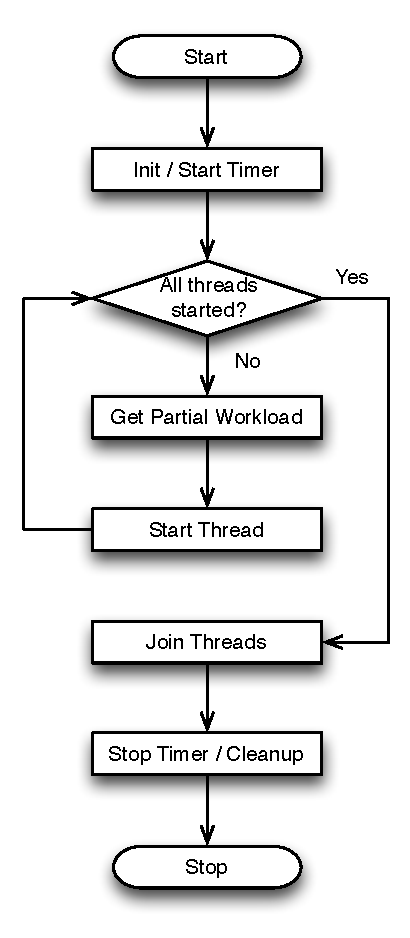
\includegraphics[width=0.75\textwidth]{figures/bench/host}
    \caption{Logical flow of the\\benchmark application.}
    \label{fig:eval-host}
\end{minipage}
\begin{minipage}[c]{0.45\linewidth}
    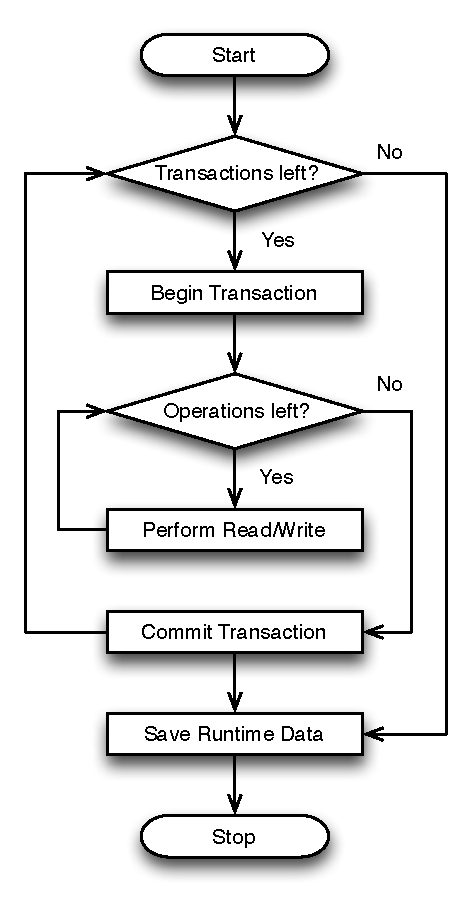
\includegraphics[width=0.89\textwidth]{figures/bench/worker}
    \caption{Logical flow of a single worker thread.}
    \label{fig:eval-worker}
\end{minipage}
\end{figure}

\subsection{Results and Discussion}

In this subsection the results of the benchmark are shown and discussed. The
benchmark captures two metrics: transaction throughput and the transaction abort
rate. In order to express the scalability of both KVS, throughput is expressed
in terms of speedup factor. This also helps comparing the performance of both
stores even if absolute throughput differs significantly. The abort rate is
given by the ratio of the number of aborted transactions and the number of
scheduled transactions. When interpreting throughputs and speedup factors, it is
important to take the abort rate into account because higher abort rates can
lead to higher transaction throughputs. The reason for this circumstance is that
commits are very expensive and the resulting time saving of an abort has a
stronger influence on throughput than reducing the number of committed
transactions. This is also a direct consequence of the two-level store
architecture and the additional measures to preserve consistency in NVRAM.

\paragraph{Legend}

The following analysis compares benchmark results of Echo (green), Midas (blue)
and its optimized variant, denoted as Midas$^{*}$ (red). In the current
implementation of Midas, the index is based on a naive hash table implementation
for NVRAM. In order to protect critical sections in the hash table, a simple
global locking mechanism is used. This approach forms a major bottleneck which
can be addressed with a designated but often complicated concurrent design as in
\cite{fan2013memc3}. However, this is an implementation detail, albeit crucial.
In order to show the potential of Midas' design, a second variant of Midas
without index locking was examined. This is possible because during the
benchmark not the index but only histories are modified. This is a side effect
of omitting insert and delete operations for simplicity.

\newcommand{\midasopt}{Midas$^{*}$\xspace}
\newcommand{\midas}{Midas\xspace}
\newcommand{\echo}{Echo\xspace}
\newcommand{\ttp}{transaction throughput\xspace}
\newcommand{\tput}{throughput\xspace}
\newcommand{\eff}{parallel efficiency\xspace}

%==============================================================================
% [1 = SS]
%==============================================================================

\clearpage

\paragraph{Scenario S1}

This scenario simulates high contention by means of a small database but short
transactions. The expected outcome in this scenario is that \echo performs
better than \midas because it detects fewer conflicts which are also less
likely. At first, the plot of \ttp in Figure \ref{fig:ttp-s1} confirms that
expectation. However, it also confirms that the index lock in \midas is a
massive bottleneck as \midasopt achieves up to 50\% higher \tput than \echo.
Concerning speedup factors, all stores fail to improve for more than 8 cores
(see Figure \ref{fig:spd-s1}). This is better reflected in terms of \eff as
shown in Figure \ref{fig:eff-s1}. The reason is that there are very few
key-value pairs which increases synchronization overhead. As expected, both
variants of \midas exhibit much higher abort rates than \echo, due to stricter
conflict detection (see Figure \ref{fig:ar-s1}). While \midasopt makes the best
use of additional cores, it produces a slightly higher abort rate than \midas.
This reveals a serializing nature of the global lock in the original
implementation of \midas.

\begin{figure}[h!]
\begin{minipage}[l]{0.50\textwidth}
    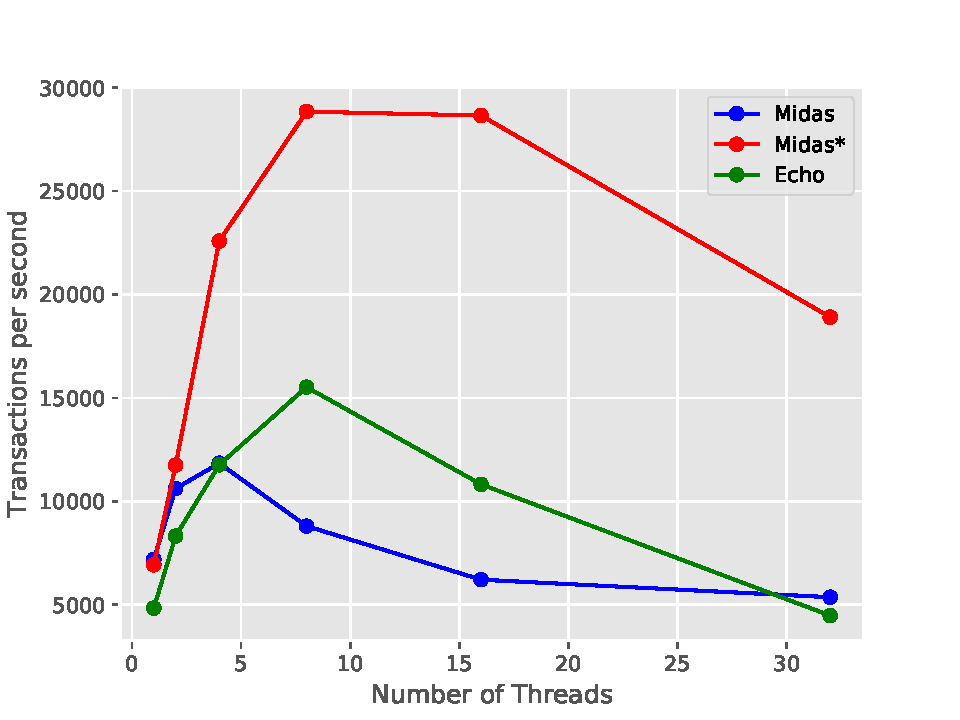
\includegraphics[width=\textwidth]{figures/bench/ttp-ss}
    \caption{Transaction throughput for\\scenario S1.}
    \label{fig:ttp-s1}
\end{minipage}
\begin{minipage}[l]{0.50\textwidth}
    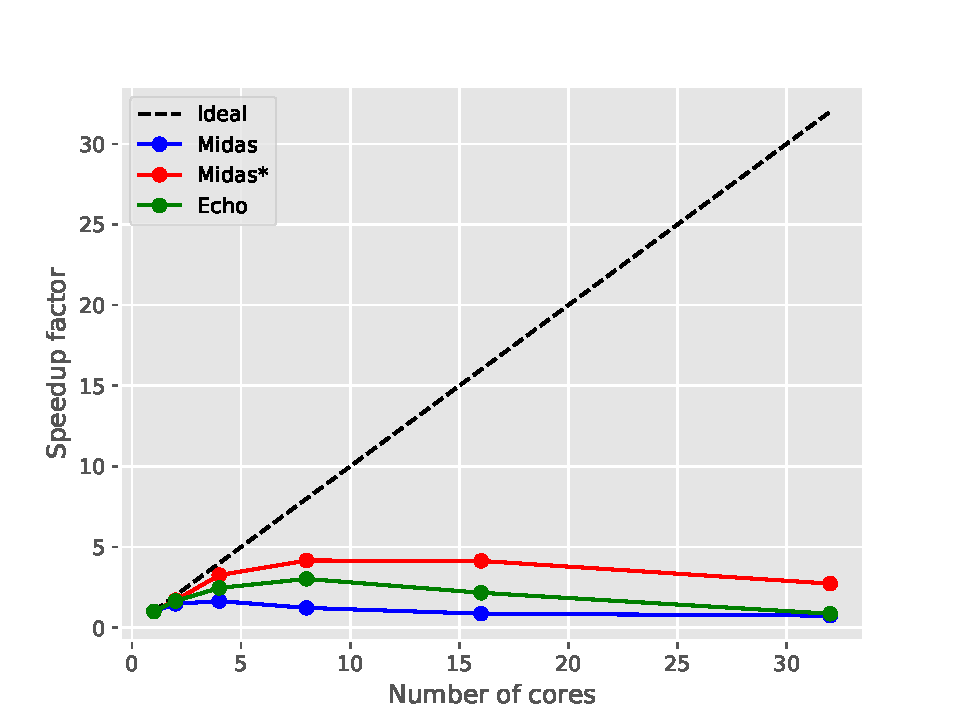
\includegraphics[width=\textwidth]{figures/bench/spd-ss}
    \caption{Transaction throughput speedup for scenario S1.}
    \label{fig:spd-s1}
\end{minipage}
\begin{minipage}[l]{0.50\textwidth}
    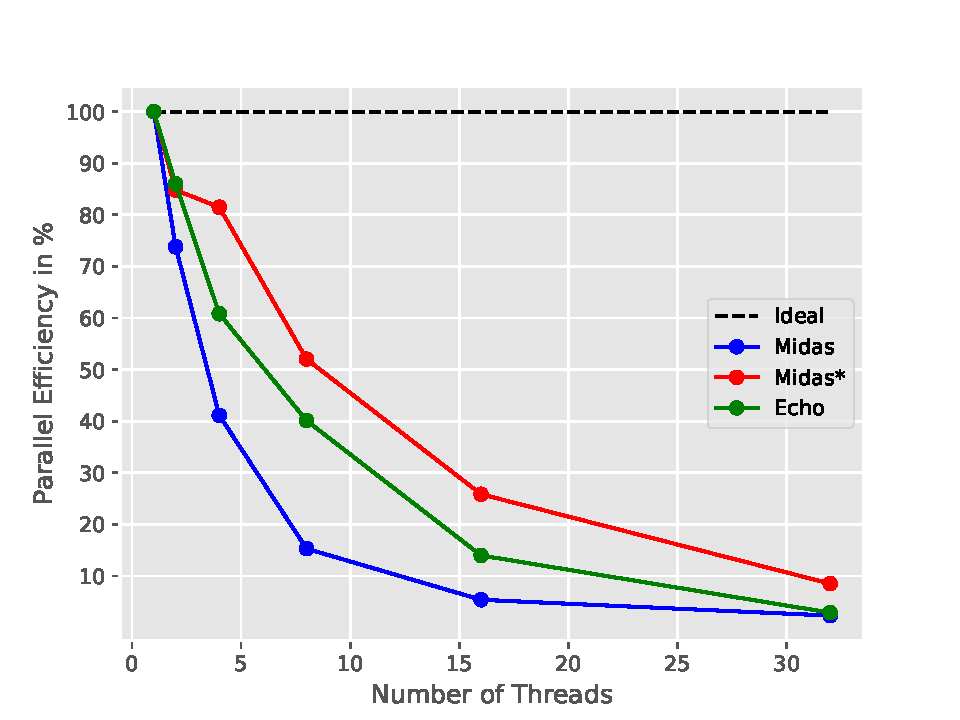
\includegraphics[width=\textwidth]{figures/bench/eff-ss}
    \caption{Parallel efficiency for scenario S1.}
    \label{fig:eff-s1}
\end{minipage}
\begin{minipage}[l]{0.50\textwidth}
    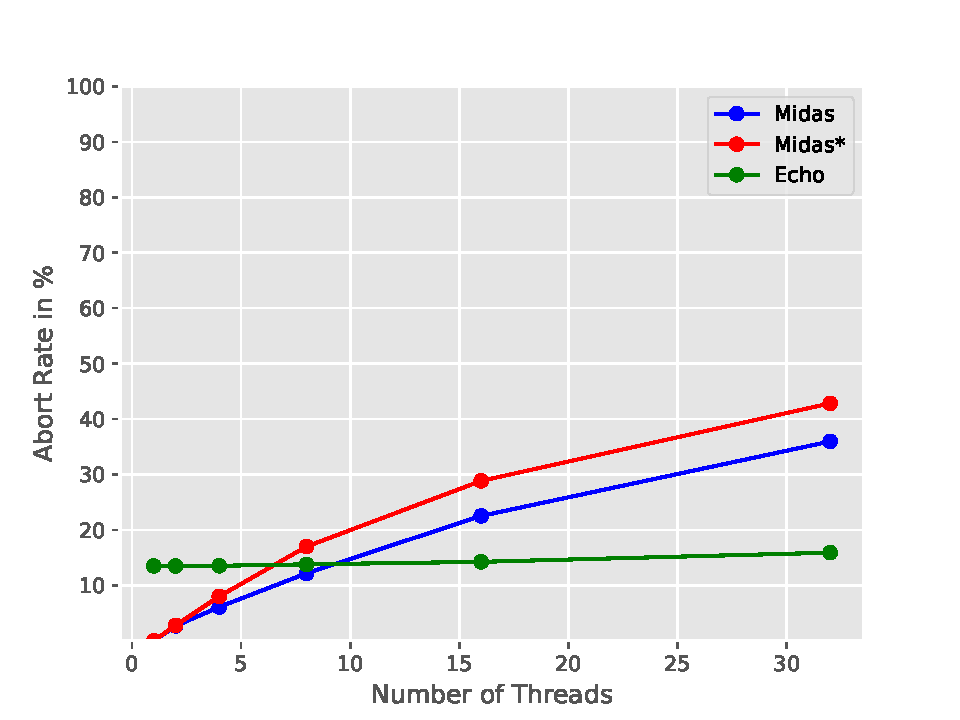
\includegraphics[width=\textwidth]{figures/bench/ar-ss}
    \caption{Abort rate for scenario S1.}
    \label{fig:ar-s1}
\end{minipage}
\end{figure}

%==============================================================================
% [2 = SL]
%==============================================================================

\paragraph{Scenario S2}

This scenario simulates very high contention by means of a small database and
long transactions. It can be seen as the worst-case scenario for concurrency
controls with strong isolation levels. Therefore, both versions of \midas are
expected to be outperformed by \echo. The plot in Figure \ref{fig:ttp-s2}
confirms that, as \ttp for both \midas and \midasopt plummets towards zero. This
is also reflected in speedup factors and \eff in Figures \ref{fig:spd-s2} and
\ref{fig:eff-s2}. Unlike in the previous scenario, this result is dominated by
extreme abort rates approaching 100\% which can be seen in Figure
\ref{fig:ar-s2}. Note that \midasopt, despite committing almost no transactions,
still shows some \tput at 32 cores because it has less synchronization overhead
than \midas and saved time by not committing. \echo, on the other hand, has much
lower abort rates. This results in significantly better \ttp at first, but, starting at 8 cores, \tput starts to decline rapidly as well.

\begin{figure}[h!]
\begin{minipage}[l]{0.50\textwidth}
    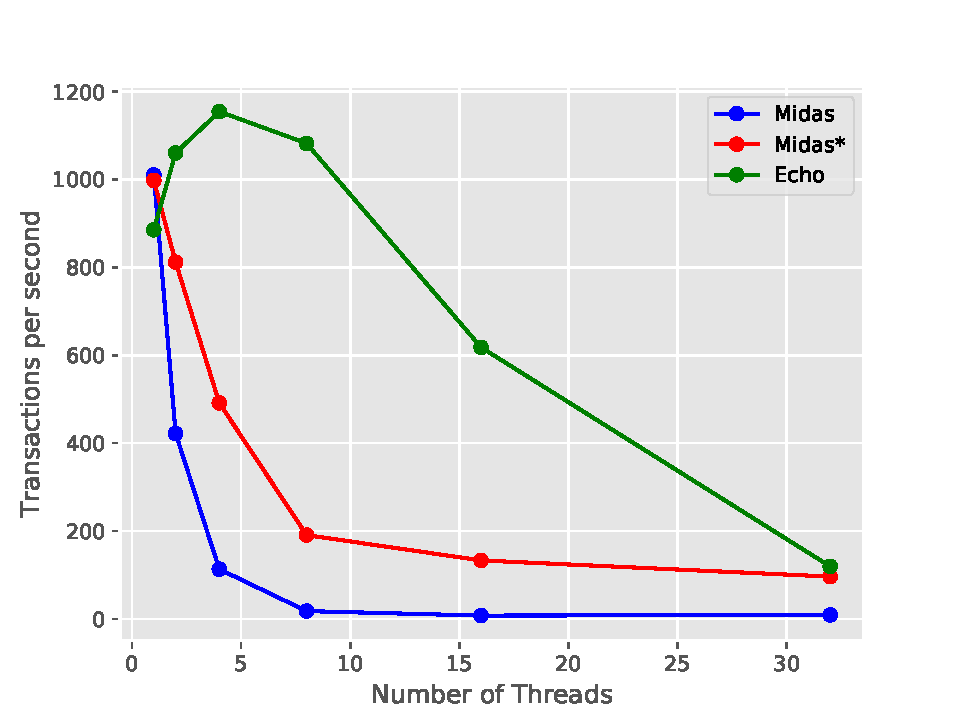
\includegraphics[width=\textwidth]{figures/bench/ttp-sl}
    \caption{Transaction throughput for\\scenario S2.}
    \label{fig:ttp-s2}
\end{minipage}
\begin{minipage}[l]{0.50\textwidth}
    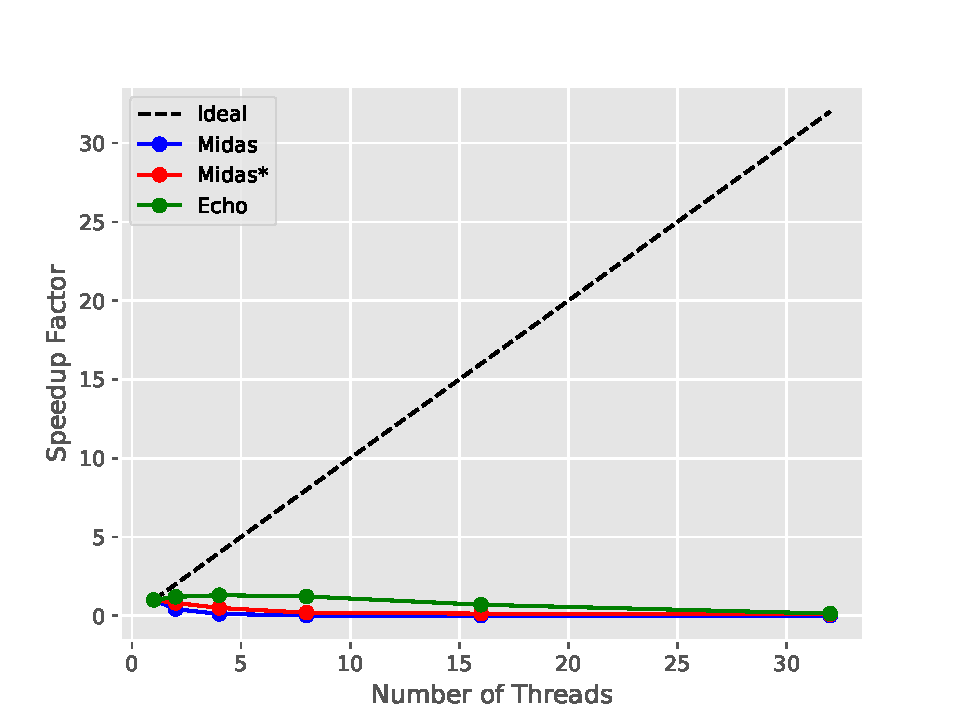
\includegraphics[width=\textwidth]{figures/bench/spd-sl}
    \caption{Transaction throughput speedup for scenario S2.}
    \label{fig:spd-s2}
\end{minipage}
\begin{minipage}[l]{0.50\textwidth}
    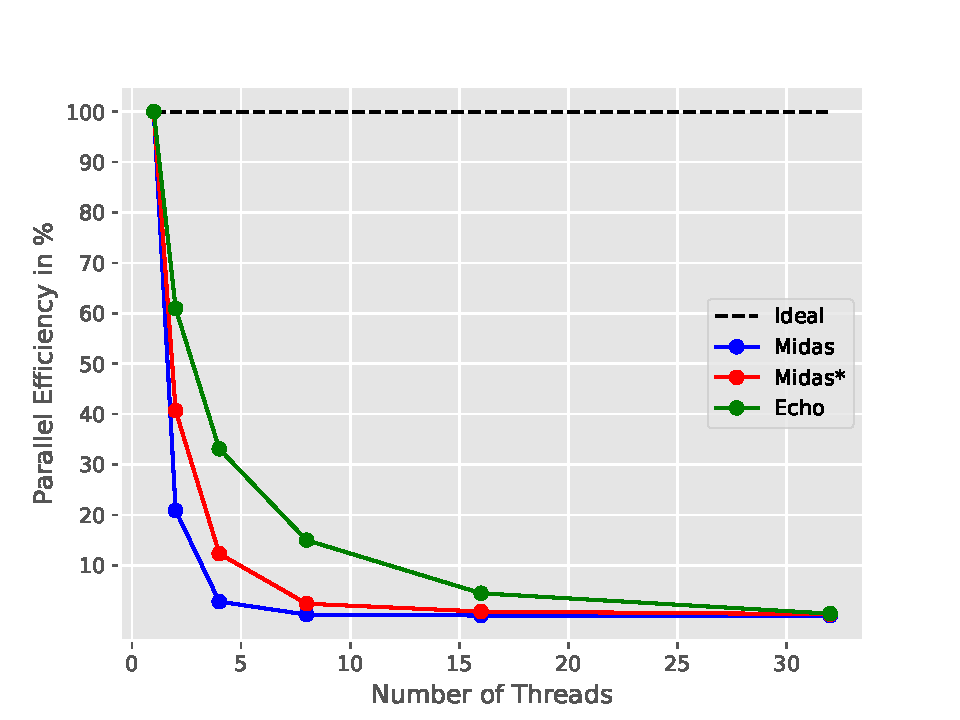
\includegraphics[width=\textwidth]{figures/bench/eff-sl}
    \caption{Parallel efficiency for scenario S2.}
    \label{fig:eff-s2}
\end{minipage}
\begin{minipage}[l]{0.50\textwidth}
    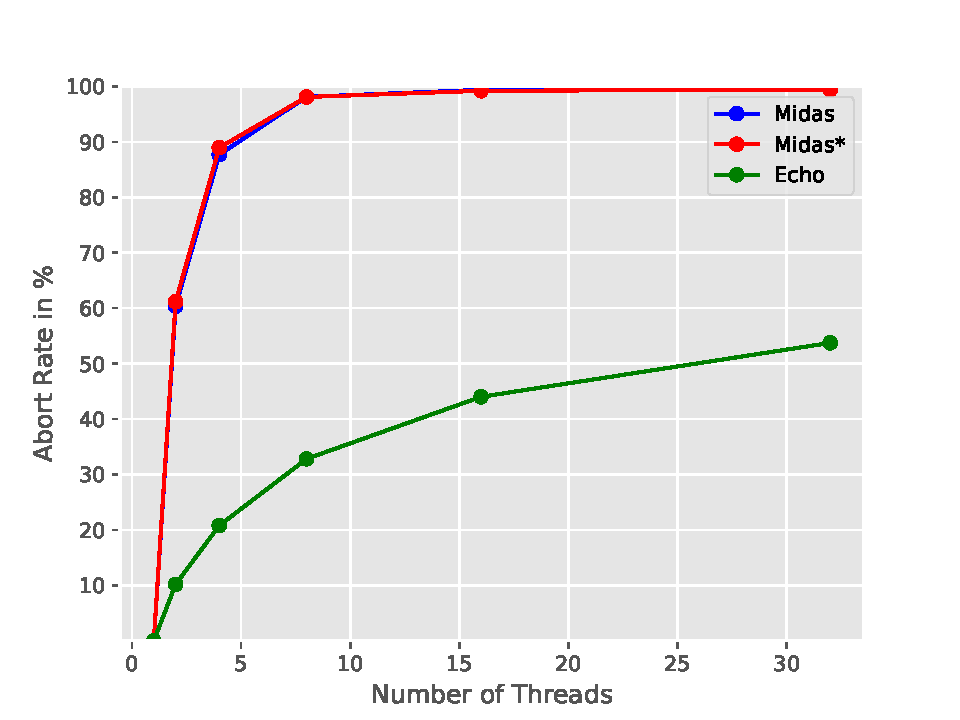
\includegraphics[width=\textwidth]{figures/bench/ar-sl}
    \caption{Abort rate for scenario S2.}
    \label{fig:ar-s2}
\end{minipage}
\end{figure}

%==============================================================================
% [3 = LS]
%==============================================================================

\paragraph{Scenario S3}

This scenario simulates low contention by means of a large database and short
transactions. Based on the lower probability of conflicts, it is expected that
\midas could be on a par with \echo. The plot in Figure \ref{fig:ttp-s3} shows
that \ttp in both \midas and \midasopt is significantly higher than in \echo.
While \midas is too limited by synchronization to benefit from additional cores,
\echo and \midasopt achieve close-to-ideal speedup until 4 cores (see Figure
\ref{fig:spd-s3} and \ref{fig:eff-s3}). Beyond that, \echo starts plunging at 8
cores whereas \midasopt manages to improve until 16 cores, albeit slightly.

\begin{figure}[h!]
\begin{minipage}[l]{0.50\textwidth}
    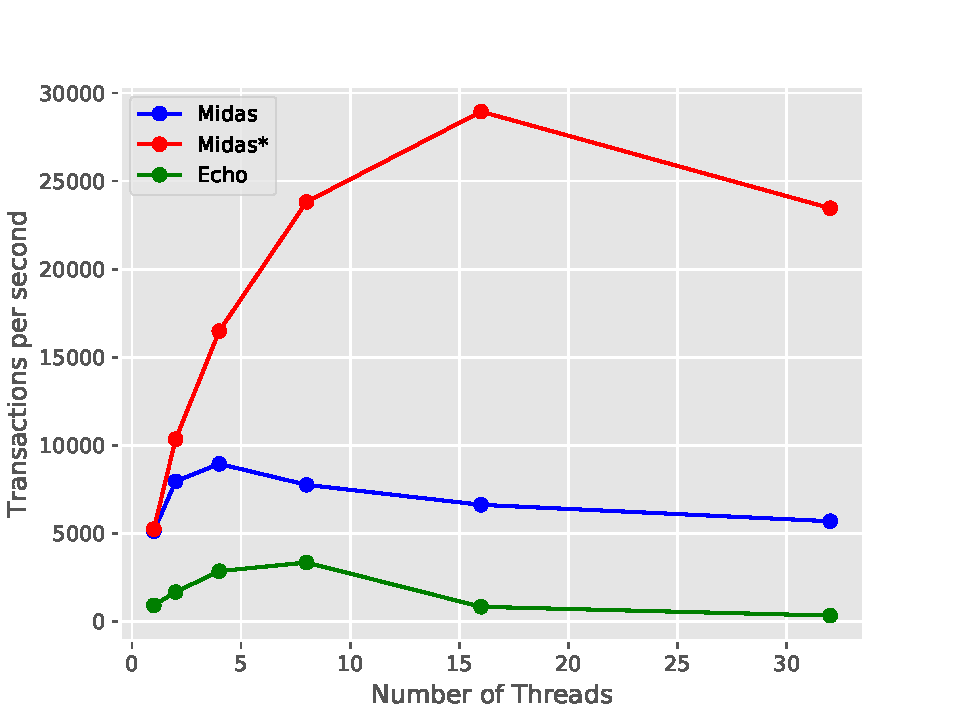
\includegraphics[width=\textwidth]{figures/bench/ttp-ls}
    \caption{Transaction throughput for\\scenario S3.}
    \label{fig:ttp-s3}
\end{minipage}
\begin{minipage}[l]{0.50\textwidth}
    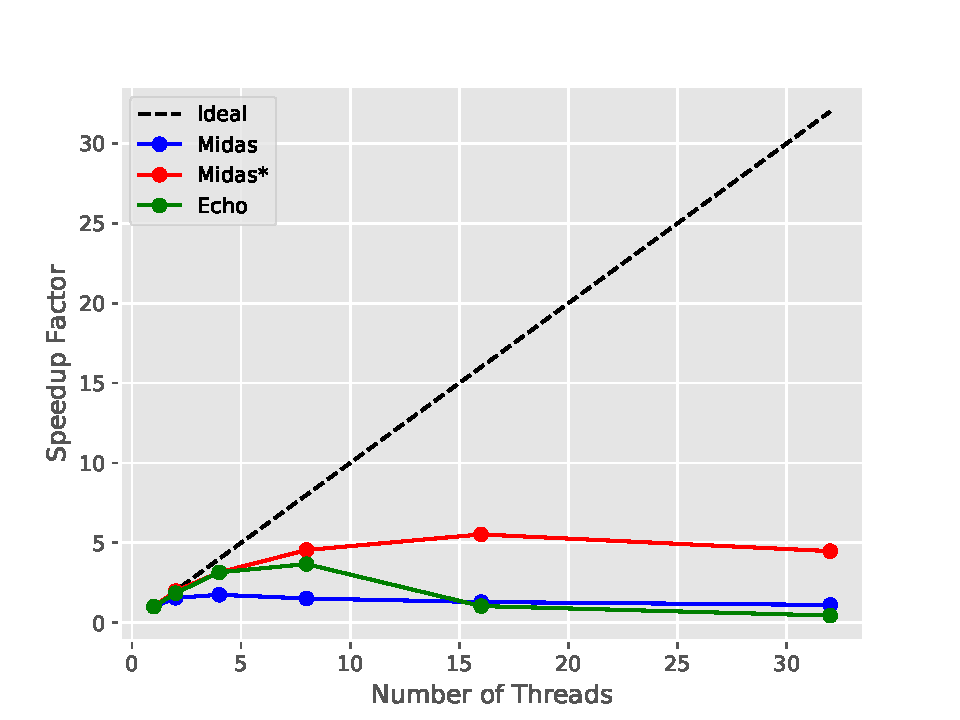
\includegraphics[width=\textwidth]{figures/bench/spd-ls}
    \caption{Transaction throughput speedup for scenario S3.}
    \label{fig:spd-s3}
\end{minipage}
\begin{minipage}[l]{0.50\textwidth}
    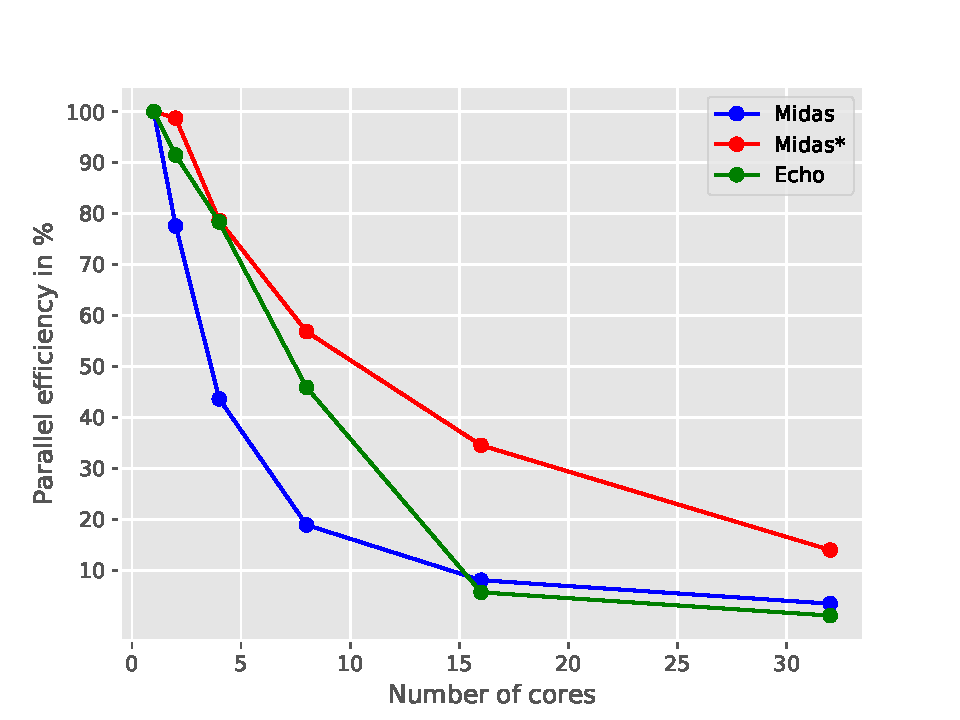
\includegraphics[width=\textwidth]{figures/bench/eff-ls}
    \caption{Parallel efficiency for scenario S3.}
    \label{fig:eff-s3}
\end{minipage}
\begin{minipage}[l]{0.50\textwidth}
    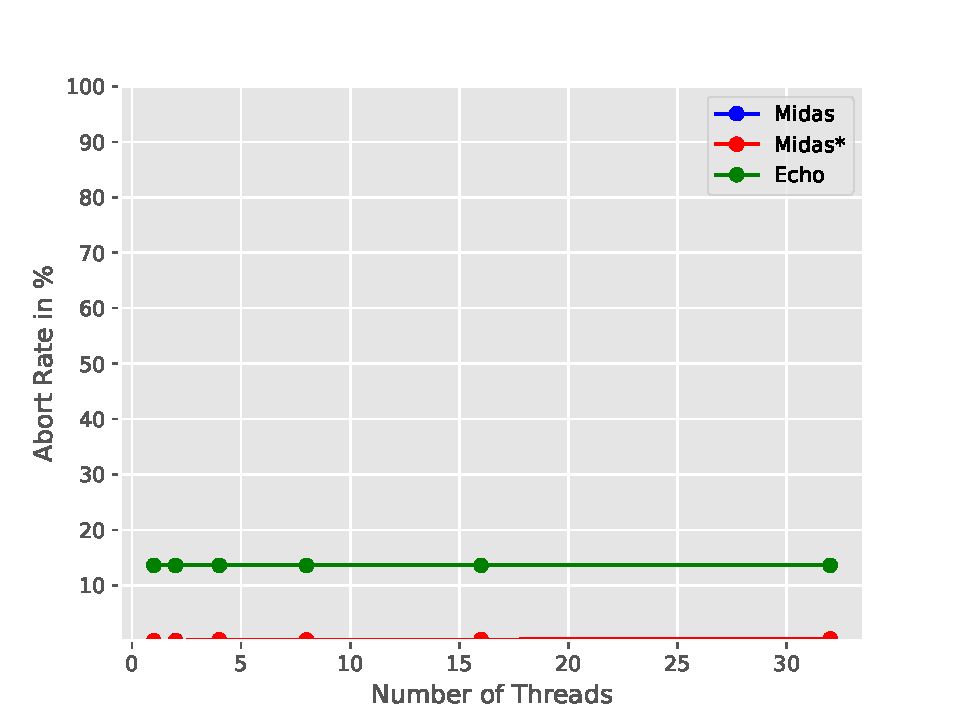
\includegraphics[width=\textwidth]{figures/bench/ar-ls}
    \caption{Abort rate for scenario S3.}
    \label{fig:ar-s3}
\end{minipage}
\end{figure}

This is a significant result, because it shows that serializable MVCC can still
perform well for workloads where SI is known to excel at. After all, \midasopt
manages to surpass \echo by a large margin. However, Figure \ref{fig:ar-s3}
shows that this scenario appears to be well-natured for strong isolation as
abort rates are consistently below 1\%. A side effect is that \ttp values cannot
be distorted by time savings from aborted transactions. Also, the unsynchronized
index in \midasopt surely is too optimistic for an approximation of a concurrent
index.

% However, it must be noted, that other factors may play a
% role. For instance, \echo and \midas use different backends to handle potential
% NVRAM. Also, the optimized variant of \midas does not synchronize access to its
% index, which is a very optimistic approximation of a non-blocking concurrent
% implementation.

%==============================================================================
% [4 = LL]
%==============================================================================

\paragraph{Scenario S4}

The last scenario simulates medium contention by means of a large database
accessed by long transactions. This scenario is similar to S3 but the longer
transactions access the index more often and make aborts more likely, which is a
disadvantage for \midas. This circumstance is confirmed in Figure
\ref{fig:ttp-s4} as \echo achieves higher \ttp than \midas. Also, \echo scales
better than \midas which is depicated in Figures \ref{fig:spd-s4} and
\ref{fig:eff-s4}.

\begin{figure}[h!]
\begin{minipage}[l]{0.50\textwidth}
    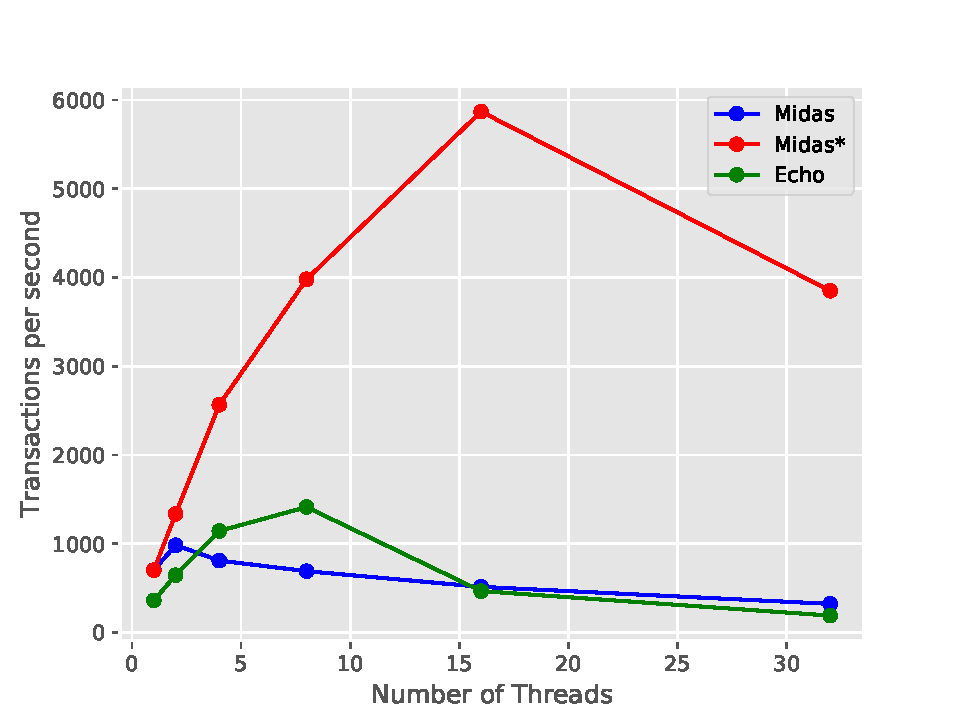
\includegraphics[width=\textwidth]{figures/bench/ttp-ll}
    \caption{Transaction throughput for\\scenario S4.}
    \label{fig:ttp-s4}
\end{minipage}
\begin{minipage}[l]{0.50\textwidth}
    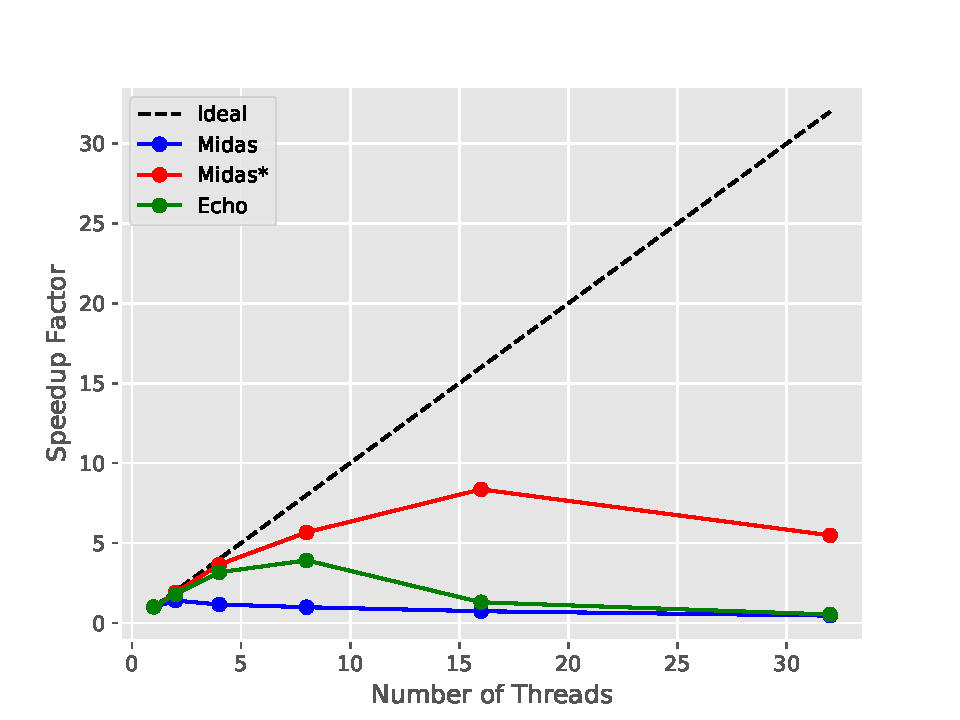
\includegraphics[width=\textwidth]{figures/bench/spd-ll}
    \caption{Transaction throughput speedup for scenario S4.}
    \label{fig:spd-s4}
\end{minipage}
\begin{minipage}[l]{0.50\textwidth}
    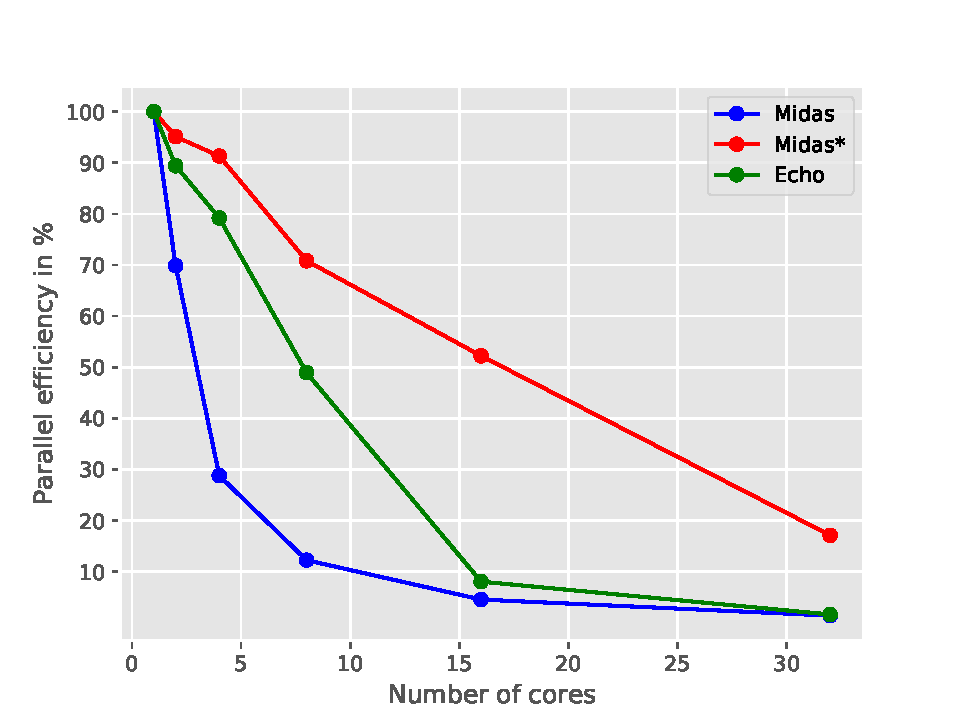
\includegraphics[width=\textwidth]{figures/bench/eff-ll}
    \caption{Parallel efficiency for scenario S4.}
    \label{fig:eff-s4}
\end{minipage}
\begin{minipage}[l]{0.50\textwidth}
    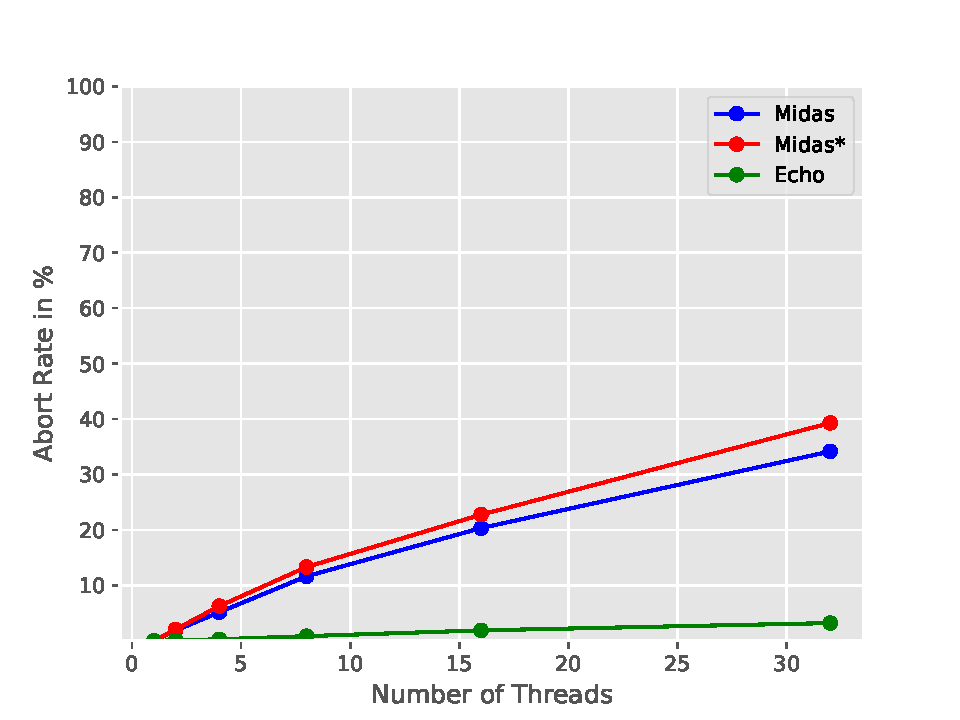
\includegraphics[width=\textwidth]{figures/bench/ar-ll}
    \caption{Abort rate for scenario S4.}
    \label{fig:ar-s4}
\end{minipage}
\end{figure}

\clearpage

However, this is largely attributed to synchronization overhead in \midas, as
\midasopt achieves up to 6 times higher \tput than \echo while it produces only
slightly higher abort rates (see Figures \ref{fig:ttp-s4} and \ref{fig:ar-s4}).
Note that \midasopt shows even better speedups than in scenario S3, but that is
most likely due to time savings from aborted transactions which are more
numerous in S4. A troubling observation from Figure \ref{fig:ar-s4} is that,
longer transactions alone can cause abort rates to scale in the number of cores
for both variants of \midas. Independent of high abort rates, \ttp in \midasopt
suddently declines rapidly at 32 cores. A possible explanation is that remaining
synchronization points in \midasopt incur too much overhead to be compensated by
time savings from aborted transactions. \echo, on the other hand, has
significantly fewer aborts but cannot exploit the advantage as it fails to
leverage more than 8 cores efficiently.
